
\documentclass[conference]{IEEEtran}
% If the IEEEtran.cls has not been installed into the LaTeX system files, 
% manually specify the path to it: e.g.,
% \documentclass[conference]{../sty/IEEEtran} 

\usepackage{graphicx,times,amsmath} % Add all your packages here

% correct bad hyphenation here
\hyphenation{op-tical net-works semi-conduc-tor IEEEtran}

\IEEEoverridecommandlockouts	% to create the author's affliation portion
				% using \thanks
				
\textwidth 178mm   	% <------ These are the adjustments we made 10/18/2005
\textheight 239mm	% You may or may not need to adjust these numbes again
\oddsidemargin -7mm
\evensidemargin -7mm
\topmargin -6mm 
\columnsep 5mm

\begin{document}


% paper title: Must keep \ \\ \LARGE\bf in it to leave enough margin.
\title{\ \\ \LARGE\bf Sample Paper for CEC 2007: The IEEE 
 Congress on Evolutionary Computation\thanks{K. C. Tan is with the
Department of Electrical and Computer Engineering,National University of Singapore, 4 Enginnering Drive 3, Sinagpore
(phone: 65-6516-2721; fax: 65-6779-1103; email: eletankc@nus.edu.sg).}
}

\author{K. C. Tan, {\it Member, IEEE}}
% avoiding spaces at the end of the author lines is not a problem with
% conference papers because we don't use \thanks or \IEEEmembership
% use only for invited papers
%\specialpapernotice{(Invited Paper)}

% make the title area
\maketitle

\begin{abstract}
The abstract goes here. What you need to do is to insert your abstract
here. Please try to make it less than 150 words. 
We suggest that you read this document carefully before you begin preparing
your manuscript. IEEE does not want conference papers to have 
keywords so you should remove your keyword list. 
Also, at this time, IEEE only has some general guidelines about the 
format for conference papers.
It is up to each individual conference to decide which format to use.
In order to have a uniform look for all papers published in the CEC 
2007 Proceeding, we require that every author follow the 
format of this sample paper.  This sample paper is for latex users. 
Authors may use the sample paper here to produce their own 
papers by following the same format as this sample paper.
\end{abstract}

% no key words

\section{Introduction}
% no \PARstart

If you have an introduction for your paper, put it here.
This sample file is intended to serve as a ``starter file."
You need to cut out our text and then insert your text into this file.

\subsection{Subsection Heading Here}
Note that you need to use $\backslash$subsection.
Subsection text goes here, if applicable.
You may or may not have any subsections. That is OK.

\subsubsection{Subsubsection Heading}
Insert subsubsection text here.
Same thing, you may or may not have any subsubsections. That is fine.

\subsubsection{About This Template}
This sample paper is for latex users. Authors may use the sample paper 
here to produce their own paper.
WORD users can also download the template file for WORD posted on the
CEC 2007 website.

\subsection{Page layout}
\begin{itemize}
\item IEEE now only accepts 100$\%$ 
	Xplore compliant papers prepared in PDF format. Please make sure that 
	you follow these guidelines in preparing 
	your PDF files. Violations of any of these specifications 
	may result in rejection of your papers.  
\item Paper size: US letter format ($8.5\times 11$ in) 
or $216\times 278$ mm.
\item File size limitation: 2.0 MB.
\item Paper length: %Minimum 4 pages and m
Maximum 8 pages, including figures, tables and references.
In exceptional circumstances up to two additional pages will be
permitted for a charge of \$150 per additional page.
\item Paper formatting: Double column, single spaced, 10pt font.
\item Text width: 7.0 in (178 mm) and text height: 9.375 in (240 mm).

All text and figures must be contained in the $178 \times 240$ mm  image area.
\item The left/right/bottom margin must be 0.75 in (19 mm).
\item The top margin must be 0.75 in (19 mm),
 except for the title page where it must be 1 in (25 mm).
\item Text should appear in two columns, each 3.4 in (86.5 mm) wide with 0.2 in
(5 mm) space between columns.
%\item On the first page, the top 50 mm (2 in) of both columns is reserved for 
%the title, author(s), and affiliation(s) as shown in this sample paper. 
%These items should be centered across both columns, starting at 35 mm 
%(1.375 inches) from the top of the page.
\item Do NOT page number your manuscript.
\item Unix LaTeX users please use the following command:
\begin{itemize}
\item latex mypaper
\item dvips -Ppdf -G0 -tletter mypaper.dvi
\item ps2pdf mypaper.ps mypaper.pdf
\end{itemize}
\end{itemize}
    
The page size and margin settings in IEEEtran.cls are set for 
IEEE Transactions papers. We have made some adjustments to 
produce this sample paper.

{\it Also, please note that IEEE PDF eXpress will be made available to assist you in 
creating the IEEE Xplore compliant PDF file for the camera-ready submissions.}

% An example of a double column floating figure using two subfigures.
%(The subfigure.sty package must be loaded for this to work.)
% The subfigure \label commands are set within each subfigure command, the
% \label for the overall fgure must come after \caption.
% \hfil must be used as a separator to get equal spacing
%
%\begin{figure*}
%\centerline{\subfigure[Case I]{\includegraphics[width=2.5in]{subfigcase1}
% where an .eps filename suffix will be assumed under latex, 
% and a .pdf suffix will be assumed for pdflatex
%\label{fig_first_case}}
%\hfil
%\subfigure[Case II]{\includegraphics[width=2.5in]{subfigcase2}
% where an .eps filename suffix will be assumed under latex, 
% and a .pdf suffix will be assumed for pdflatex
%\label{fig_second_case}}}
%\caption{Simulation results}
%\label{fig_sim}
%\end{figure*}

\section{Main Results}
The main results and findings go here. You may also have a section for 
Preliminaries before this section.

First, if you do not want to number an equation, do not use
$\backslash$begin--$\backslash$end.
You can either use $\backslash$[ --$\backslash$] or
\$\$--\$\$. For example, we have
$$\dot x= f( x,u) + g (x,u)$$
or 
\[\ddot s=G(s,t)\]
where $f,$ $g,$ and $G$ are functions. It is recommended that you do not 
number an equation if it will not be cited in your paper.

Equation (\ref{eq:eq1}) is numbered!
The following equation is produced 
using $\backslash$begin\{equation\}--$\backslash$end\{equation\}.
The main objective function for each unit can be represented by a 
quadratic cost function given by
\begin{equation}
F_i(P_i)=a_{i}+b_{i}P_i+c_{i}P_{i}^2
\label{eq:eq1}
\end{equation}
where  $a_{i},\ b_{i}$, and $c_{i}$ in (\ref{eq:eq1}) are the fuel consumption cost coefficients 
of unit $i$, and $P_i$ represents the value of the power to be 
determined for unit $i$.

Recently, it is popular to use
$\backslash$begin\{align\}--$\backslash$end\{align\}
instead of
$\backslash$begin\{eqnarray\}--$\backslash$end\{eqnarray\}.
Equation (\ref{eq4b}) is produced using 
$\backslash$begin\{align\}--$\backslash$end\{align\}.
The objective function for each unit can be represented by
\begin{align}
\dot {x}_l=& \sum_{i = 1}^m {\frac{c_{P_{x_i} } e^{k_{x_i}\bar{x}_i} + c_{N_{x_i} }
e^{ -  k_{x_i} \bar{x}_i}}{e^{k_{x_i} \bar{x}_i} + e^{ - k_{x_i} \bar{x}_i}}} \nonumber\\
& + \frac{1}{2}\sum\limits_j^q (c_{P{u_j }} + c_{N _{u_j }} ) \nonumber\\
y=& \ A_0 + A_1 \tanh (K_x \bar {x}) + B\tanh (K_u \bar {u}) \nonumber\\
 =& \ F(x),\label{eq4b}
\end{align}
where $F(x)$ is a function.

Well, the same equation, when it is produced using 
$\backslash$begin\{eqnarray\}--$\backslash$end\{eqnarray\} becomes
(\ref{eq4c}):
\begin{eqnarray}
\dot {x}_l&=& \sum_{i = 1}^m {\frac{c_{P_{x_i} } e^{k_{x_i}\bar{x}_i} + c_{N_{x_i} }
e^{ - k_{x_i} \bar{x}_i}}{e^{k_{x_i} \bar{x}_i} + e^{ - k_{x_i} \bar{x}_i}}} \nonumber\\
&&+ \frac{1}{2}\sum\limits_j^q (c_{P{u_j }} + c_{N _{u_j }} ) \nonumber\\
y&=& \ A_0 + A_1 \tanh (K_x \bar {x}) + B\tanh (K_u \bar {u})\nonumber\\
&=& \ F(x),\label{eq4c}
\end{eqnarray}
where $F(x)$ is a function. You get the idea!

\subsection{Example of a Figure}
An example of a floating figure using the graphicx package.
Note that $\backslash$label must occur AFTER (or within) $\backslash$caption.
For figures, $\backslash$caption should occur after the 
$\backslash$includegraphics.
You also need to know how to cite your figure. Here is an example:
Figure~\ref{fig_sim} show our simulation results.

\begin{figure}[htp]
\centerline{\includegraphics[width=3.35in]{fig1.eps}}
\caption{Simulation results}
\label{fig_sim}
\end{figure}

\subsection{Figures and Tables}
Please follow the style in the sample paper when generating your figures and tables.

\def\del{
\subsection{What Sections to Include}
Usually, your paper should have Introduction, Main Results, Simulation Results, and
Conclusions. You may also add Acknowledgments if you like.
After that, you should have your References.}

\subsection{Page Limit and Overlength Page Charges}

A paper submitted to this conference should be prepared in a single-spaced, two-column 
format and its length must be kept to 8 pages and below.
In exceptional circumstances up to two additional pages will be
permitted for a charge of \$150 per additional page.
Table~\ref{table_example} shows the page limit
and page charge schedule.

% An example of a floating table. Note that, for IEEE style tables, the 
% \caption command should come BEFORE the table.Table text will default to
% \footnotesize as IEEE normally uses this smaller font for tables.
% The \label must come after \caption as always.
%
\begin{table}
\begin{center}
%% increase table row spacing, adjust to taste
\renewcommand{\arraystretch}{1.3}
\caption{Page Limit}
\label{table_example}
% The array package and the MDW tools package offers better commands
%% for making tables than plain LaTeX2e's tabular which is used here.
\begin{tabular}{|c|c|}
\hline
Page limits & 8\\
\hline
Excess page charge & \$150/page\\
\hline
\end{tabular}
\end{center}
\end{table}

Another example of table is shown in Table~\ref{tab-liu2}.

\begin{table}[h]
\caption{Comparison results  with methods in \cite{cit:mic77} 
(40 unit system with valve-point effects)}
\begin{center}
\begin{tabular}{|c|c|c|c|c|c|}
\hline
\multicolumn{1}{|c|}{\raisebox{-1.50ex}[0cm][0cm]{\!Method\!}}
& \multicolumn{1}{|c|}{Mean}% time}
& \multicolumn{1}{|c|}{Best}% time}
& \multicolumn{1}{|c|}{Mean}% cost}
& \multicolumn{1}{|c|}{Maximum}% cost}
& \multicolumn{1}{|c|}{Minimum} \\% cost}\\
%\hline
& time&time& cost&cost&cost\\ \hline
 CEP   &  $928.36$  &  $926.20$  &  $124793.5$ & $126902.9$ & $123488.3$ \\ \hline
 FEP   &  $646.16$  &  $644.28$  &  $124119.4$ & $127245.9$ & $122679.7$ \\ \hline
 MFEP  &  $1056.8$  &  $1054.2$  &  $123489.7$ & $124356.5$ & $122647.6$ \\ \hline
 IFEP  &  $632.67$  &  $630.36$  &  $123382.0$ & $125740.6$ & $122624.4$ \\ \hline
 TM    &  $94.28$  &  $91.16$  &  $123078.2$ & $124693.8$ & $122477.8$ \\ \hline
\end{tabular}
\label{tab-liu2}
\end{center}
\end{table}

\section{Conclusions}
The conclusion goes here.
This sample paper is for latex users. Authors may follow the sample paper here to 
produce their own 
papers by following the same format as this sample paper.

% conference papers do not normally have an appendix

% use section* for appendix
\section*{Appendix}
Put your appendix here if you have any.

% use section* for acknowledgment
\section*{Acknowledgment}
% optional entry into table of contents (if used)
%\addcontentsline{toc}{section}{Acknowledgment}
The authors would like to thank Mr. XYZ for his/her help.
This work was supported in part by the National Science Foundation
under grant no. XXXXX, etc.

% trigger a \newpage just before the given reference
% number - used to balance the columns on the last page
% adjust value as needed - may need to be readjusted if
% the document is modified later
%\IEEEtriggeratref{8}
% The "triggered" command can be changed if desired:
%\IEEEtriggercmd{\enlargethispage{-5in}}

% references section
% NOTE: BibTeX documentation can be easily obtained at:
% http://www.ctan.org/tex-archive/biblio/bibtex/contrib/doc/

% can use a bibliography generated by BibTeX as a .bbl file
% standard IEEE bibliography style from:
% http://www.ctan.org/tex-archive/macros/latex/contrib/supported/IEEEtran/testflow/bibtex
%\bibliographystyle{IEEEtran.bst}
% argument is your BibTeX string definitions and bibliography database(s)
%\bibliography{IEEEabrv,../bib/paper}
%
% <OR> manually copy in the resultant .bbl file
% set second argument of \begin to the number of references
% (used to reserve space for the reference number labels box)


\def\V{\rm vol.~}
\def\N{no.~}
\def\pp{pp.~}
\def\Pot{\it Proc. }
\def\IJCNN{\it International Joint Conference on Neural Networks\rm }
\def\ACC{\it American Control Conference\rm }
\def\SMC{\it IEEE Trans. Systems\rm , \it Man\rm , and \it Cybernetics\rm }

\def\handb{ \it Handbook of Intelligent Control: Neural\rm , \it
    Fuzzy\rm , \it and Adaptive Approaches \rm }
                                      
\begin{thebibliography}{1}
\bibitem{cit:del2303} P. G. DeLima and G. G. Yen, 
``Multiple model fault tolerant control using globalized dual 
heuristic programming,''
{\Pot IEEE International Symposium on Intelligent Control}, 
Houston, TX, Sept. 2003, pp. 523--528. (Invited paper) 
                                        
\bibitem{cit:mic77} A. N. Michel and R. K. Miller,
        {\it Qualitative Analysis of Large Scale Dynamical Systems},
        New York: Academic Press, 1977.
	 
\bibitem{cit:pro97}  D. V. Prokhorov, \it Adaptive Critic Designs and
    Their Applications\rm  , Ph.D. Dissertation, Texas Tech University,
     Lubbock, TX, Oct.~1997.

\bibitem{Siedited} J. Si, A. Barto, W. Powell, and D. Wunsch, Editors,
	{\it Handbook of Learning and Approximate Dynamic Programming}, 
        New York: IEEE and Wiley, 2004.
                                           
\bibitem{cit:wer9213} P. J. Werbos, ``Approximate dynamic programming for
    real-time control  and neural modeling,'' in
        \handb (Chapter~13), Edited by D.~A.~White
    and D.~A.~Sofge, New York, NY: Van Nostrand Reinhold, 1992.
                                        
\bibitem{cit:wer2087} P. J. Werbos,
``Building and understanding adaptive systems: A statistical/numerical
approach to factory automation and brain research,''
{\it IEEE Transactions on Systems, Man, and Cybernetics},
vol. SMC-17, pp. 7--20, Jan./Feb. 1987.

\end{thebibliography}

% that's all folks
\end{document}
